\section{Analysis}
\label{sec:analysis}
\subsection{Regression analysis}
\subsubsection{ExperimentA1}
Plot a scatter chart with $\sqrt{gh}$ as the horizontal coordinate 
and x as the vertical coordinate based on the data from Table \ref{t1}.
And a regression analysis and linear fit was performed on the data, 
as shown in \autoref{ExperimentA1} and results in \autoref{table4}.





\begin{figure}[h]
    \centering
    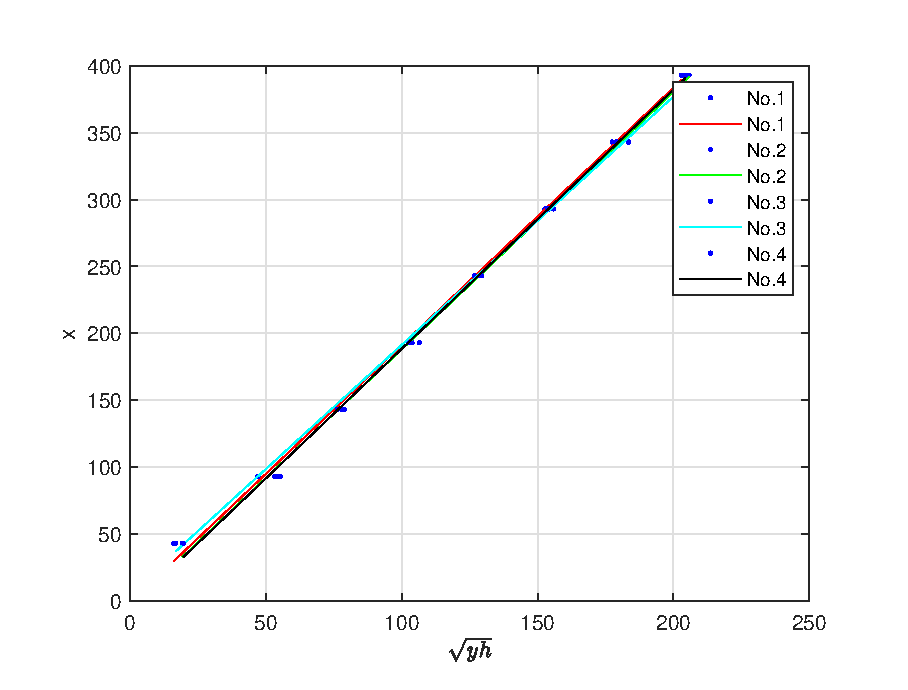
\includegraphics[width=0.75\linewidth]{Results/1.eps}
    \caption{ExperimentA1}
    \label{ExperimentA1}
    (Unit:mm)
\end{figure}

\begin{table}[h]
    \centering
    \begin{tabular}{l|ll} 
        \cline{1-3}
                             & Slope & R-square     \\ 
        \cline{1-3}
        1                    & 1.923 & 0.9968       \\
        2                    & 1.923 & 0.9976       \\
        3                    & 1.855 & 0.9985       \\
        4                    & 1.936 & 0.998        \\ 
        \cline{1-3}
        \multicolumn{1}{l}{} &       &             
        \end{tabular}
        \caption{result of A1 regression analysis}
        \label{table4}
\end{table}

Take the average of 
the data and take it into equation \eqref{6} to get $C_v=\frac{slope}{2}$.
The final $C_v$ is 0.955.

\subsubsection{ExperimentA2}
Plot a scatter chart with $\sqrt{h}$ as the horizontal coordinate 
and Q as the vertical coordinate based on the data from Table \ref{t1}.
And a regression analysis and linear fit was performed on the data, as shown in \autoref{ExperimentA2}
and results in \autoref{table5}

\begin{figure}[h]
    \centering
    \includegraphics[width=0.75\linewidth]{Results/A2.eps}
    \caption{ExperimentA2}
    \label{ExperimentA2}
    (Unit:$\sqrt{m}$ and $m^3/s$)
\end{figure}

\begin{table}[h]
    \centering
    \begin{tabular}{l|ll}
    \hline
        & Slope    & R-square \\ \hline
    3mm & 0.00001924 & 0.9955   \\
    6mm & 0.0001103 & 0.9811   \\ \hline
    \end{tabular}
    \caption{result of A2 regression analysis}
    \label{table5}
    \end{table}


Use equation \eqref{14} to caculate the $C_d=\frac{Slope}{A_0\sqrt{2g}}$
and the final $C_d$ is 0.615 (3mm)
and 0.8816 (6mm)

\subsection{Error analysis}

From the results of the regression analysis, 
the R-square value of both experiment A1 and A2 are larger than 0.98, 
which demonstrates a strong linear correlation between the x and y axes.

Therefore, the data from the regression analysis is valid.




\FloatBarrier